\section{Reduce}
\label{sec:reduce}

The next algorithm is the reduce algorithm.
The reduce algorithm is a gather operation that maps a space down to a subspace, e.g. performing a addition on an array of numbers.
The algorithm for performing parallel gathers are restricted to associative operations such that \ttt{(a op b) op c = a op (b op c)}.

\Cref{lst:reduce seq} shows the such type of operations in a serial fashion.
The operation loops through all input elements and sums the result.
The operation can be expressed such as, given $n=ARRAY\_SIZE$
\begin{equation*}
work load: O(n)
size: O(n)
\end{equation*}
\begin{lstlisting}[caption={Serial reduce}, label={lst:reduce seq}]
void reduce(int *h_in, int h_out, int SIZE) {
  for (int l = 0; l < SIZE; ++l) 
    h_out += h_in[l];
}
\end{lstlisting}

The challenge with the reduce code is that we perform all operations on a single memory address.
If the serial code is naively made parallel we would be faced with race conditions.
Instead we can look at the associative property of out problem, such that $((a+b)+c)+d = A + B$ where $A=a+b$ and $B=c+d$.
By utilizing this property we can perform the computation of $A$ and $B$ in parallel and thus halve the problem by allowing each thread to compute two numbers to one.
Reducing the problem size by a factor of two at each step gives a step size of $O(lg_2n)$ and allows us to compute parts of the problem in parallel.
We present an illustration in \cref{fig:reduce decomp example} to try to give an intuition of how the parallel code will run.~\cite{reduceharris}

\begin{figure}[htb]
  \centering
  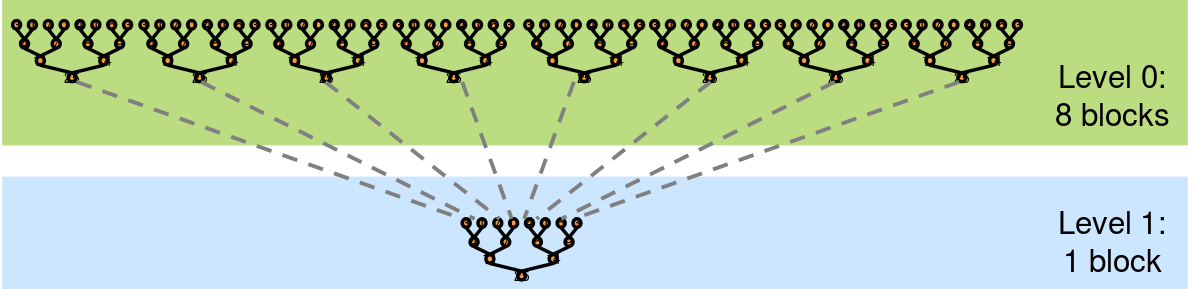
\includegraphics[width=.8\textwidth]{images/reduce_decomp_example.png}
  \caption{Reducing over multiple sweeps}
  \label{fig:reduce decomp example}
\end{figure}

The idea is that each block in the image is performed by each kernel invocation.
\Cref{lst:reduce par} shows the reduce kernel.
The needed indices are calculated, followed by the block's reduction in the loop.
Before proceeding the code makes sure that all threads have finished.
Finally, only the first thread writes the block's reduction to the output array.
The output is written to the block's index in the grid, which makes sure that each block's result is written to independent addresses.

\begin{lstlisting}[caption={Reduce kernel}, label={lst:reduce par}]
__global__
void reduce_kernel(int *d_out, int *d_in, int SIZE) {
  int mid = threadIdx.x + blockIdx.x * blockDim.x,
      tid = threadIdx.x;

  for (int s = blockDim.x / 2; s > 0; s /= 2) {
    if ((tid < s) && ((mid + s) < SIZE))
      d_in[mid] += d_in[mid + s];
    __syncthreads();
  }

  if ((tid == 0) && (mid < SIZE))
    d_out[blockIdx.x] = d_in[mid];
}
\end{lstlisting}

The intermediate results are thus transferred to the next iteration of kernel invocations.
We add a wrapper function, in \cref{lst:reduce wrapper}, that runs these kernels iteratively.
We introduce temporary arrays to hold the intermediate results, and update the grid size number of elements accordingly before invoking the kernel again.
Finally, the code performs a final invocation of the kernel with the desired final output array to combine the results.

\begin{lstlisting}[caption={The loop in the wrapper for the reduce kernel}, label={lst:reduce wrapper}]
do {
  reduce_kernel<<<grid_size, BLOCK_SIZE>>>(d_tmp_out, d_tmp_in, size);
  // Updating intermediate arrays
  size  = grid_size;
  bytes = sizeof(int) * size;
  cudaMemcpy(d_tmp_in, d_tmp_out, bytes, cudaMemcpyDeviceToDevice);
  // Updating to reflect how many blocks we now want to compute on
  grid_size = size / BLOCK_SIZE + ((size % BLOCK_SIZE)?1:0);
} while(size > BLOCK_SIZE);
// Computing remainder
reduce_kernel<<<1, size>>>(d_out, d_tmp_out, size);
\end{lstlisting}

\subsection{Using Shared Memory}
\label{sec: reduce shared memory}

As the kernel relies on computation of a subtree it performs several read/writes to global memory.
To reduce the amount of expensive transfers from global memory we propose the usage of shared memory instead.
If we have 1024 threads per block then we will do more than 3000 read and write operations to global memory.
However, if we read the needed memory into shared memory and perform the loop on that memory, then we will do about 1000 read and write operations.
Thus, we can achieve a theoretical 3x speed up.
The number of read and writes are presented in \cref{tab:reduce global to shared}.

\begin{table}[htb]
  \centering
  \begin{tabular}{c r | r r r r r}
    \toprule
    \multirow{2}*{global memory} & read  & 1024 & 512 & 256 & $\cdots$ & 1 \\
                                 & write &  512 & 256 & 128 & $\cdots$ & 1 \\
    \midrule
    \multirow{2}*{shared memory} & read  & 1024 & & &  &  \\
                                 & write &    1 & & &  &  \\
    \bottomrule
  \end{tabular}
  \caption{Global vs. Shared memory read and writes}
  \label{tab:reduce global to shared}
\end{table}

We present the revised reduce kernel with shared memory in \cref{lst:reduce par shared}.
We add the \ttt{sdata} array to contain the shared memory, and each thread copies the global data to that shared memory.


\begin{lstlisting}[caption={Reduce kernel using shared memory}, label={lst:reduce par shared}]
__global__
void reduce_kernel(int *d_out, int *d_in, int SIZE) {
  int mid = threadIdx.x + blockIdx.x * blockDim.x,
      tid = threadIdx.x;
  if (mid >= SIZE) return;

  extern __shared__ int sdata[]; // allocate shared memory
  sdata[tid] = d_in[mid];        // each thread loads global to shared memory
  __syncthreads();               // make sure all threads are done

  for (int s = blockDim.x / 2; s > 0; s /= 2) {
    if ((tid < s) && ((mid + s) < SIZE))
      sdata[tid] += sdata[tid + s]; // perform operations on shared memory
    __syncthreads();
  }

  if ((tid == 0) && (mid < SIZE))
    d_out[blockIdx.x] = sdata[0];   // copy shared back to global memory
}
\end{lstlisting}

\begin{lstlisting}[caption={Updated call to reduce kernel after use of shared memory}, label={lst:reduce invocation with smem}]
const unsigned int SMEM = BLOCK_SIZE * sizeof(int);
reduce_kernel<<<grid_size, BLOCK_SIZE, SMEM>>>(d_tmp_out, d_tmp_in, size);
\end{lstlisting}

Furthermore, we must update the kernel call to include the amount of shared memory to be allocated.
This is illustrated in \cref{lst:reduce invocation with smem}, where the third argument in the triple chevrons is the amount of shared memory to allocate.

In \cref{fig:reduce plot} is the run time for the reduce algorithms graphed.
The GPGPU gets an advantage when the array size to sum is large.
This is most likely due to overhead and memory transfers.
The GPGPU is superior to the CPU when it has enough work to spread out to its many SMs.

\begin{figure}[htb]
  \centering
  \section{Reduce}
\label{sec:reduce}

Another handy algorithm is the reduce algorithm.
The idea is to perform some binary operation on the collection of elements in some array, and return a single result.
This operation could for instance be a sum over all elements, where the operation would be addition.
The operation must be associative, i.e. \ttt{(a op b) op c = a op (b op c)}, for the reduce algorithm to perform correctly.
\Cref{lst:reduce seq} shows the serial reduce code.
The operation loops through all input elements and sums the result.

\begin{lstlisting}[caption={Serial reduce}, label={lst:reduce seq}]
void reduce(int *h_in, int h_out, int SIZE) {
  for (int l = 0; l < SIZE; ++l) 
    h_out += h_in[l];
}
\end{lstlisting}

The challenge with the reduce code is that we perform all operations on a single memory address.
If the serial code is naively made parallel we have a race condition.
We need to split the problem into smaller problems and perform several sweeps on the results and combine the intermediary results to get the final result.
We present an illustration in \cref{fig:reduce decomp example} to try to give an intuition of how the parallel code will run.~\cite{reduceharris}

\begin{figure}[htb]
  \centering
  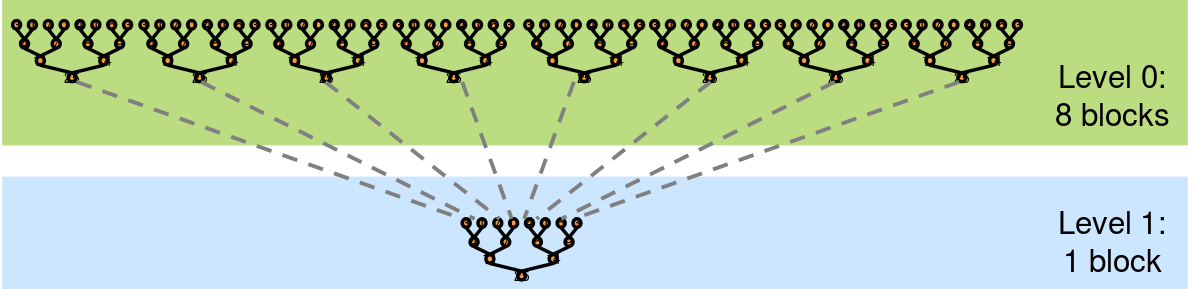
\includegraphics[width=.8\textwidth]{images/reduce_decomp_example.png}
  \caption{Reducing over multiple sweeps}
  \label{fig:reduce decomp example}
\end{figure}

The idea is that each block in the image is performed by each kernel invocation.
\Cref{lst:reduce par} shows the reduce kernel.
The needed indices are calculated, followed by the block's reduction in the loop.
Before proceeding the code makes sure that all threads have finished.
Finally, only the first thread writes the block's reduction to the output array.
The output is written to the block's index in the grid, which makes sure that each block's result is written to independent addresses.

\begin{lstlisting}[caption={Reduce kernel}, label={lst:reduce par}]
__global__
void reduce_kernel(int *d_out, int *d_in, int SIZE) {
  int mid = threadIdx.x + blockIdx.x * blockDim.x,
      tid = threadIdx.x;

  for (int s = blockDim.x / 2; s > 0; s /= 2) {
    if ((tid < s) && ((mid + s) < SIZE))
      d_in[mid] += d_in[mid + s];
    __syncthreads();
  }

  if ((tid == 0) && (mid < SIZE))
    d_out[blockIdx.x] = d_in[mid];
}
\end{lstlisting}

The intermediate results are thus transferred to the next iteration of kernel invocations.
We add a wrapper function, in \cref{lst:reduce wrapper}, that runs these kernels iteratively.
We introduce temporary arrays to hold the intermediate results, and update the grid size number of elements accordingly before invoking the kernel again.
Finally, the code performs a final invocation of the kernel with the desired final output array to combine the results.

\begin{lstlisting}[caption={The loop in the wrapper for the reduce kernel}, label={lst:reduce wrapper}]
do {
  reduce_kernel<<<grid_size, BLOCK_SIZE>>>(d_tmp_out, d_tmp_in, size);
  // Updating intermediate arrays
  size  = grid_size;
  bytes = sizeof(int) * size;
  cudaMemcpy(d_tmp_in, d_tmp_out, bytes, cudaMemcpyDeviceToDevice);
  // Updating to reflect how many blocks we now want to compute on
  grid_size = size / BLOCK_SIZE + ((size % BLOCK_SIZE)?1:0);
} while(size > BLOCK_SIZE);
// Computing remainder
reduce_kernel<<<1, size>>>(d_out, d_tmp_out, size);
\end{lstlisting}

\subsection{Using Shared Memory}
\label{sec: reduce shared memory}

A rather quick optimisation is to use shared memory instead of global memory in the kernel.
The kernel performs read and write operations in the l
If we have 1024 threads per block then we will do more than 3000 read and write operations to global memory.
However, if we read the needed memory into shared memory and perform the loop on that memory, then we will do about 1000 read and write operations.
Thus, we can achieve a theoretical 3x speed up.
The number of read and writes are presented in \cref{tab:reduce global to shared}.

\begin{table}[htb]
  \centering
  \begin{tabular}{c r | r r r r r}
    \toprule
    \multirow{2}*{global memory} & read  & 1024 & 512 & 256 & $\cdots$ & 1 \\
                                 & write &  512 & 256 & 128 & $\cdots$ & 1 \\
    \midrule
    \multirow{2}*{shared memory} & read  & 1024 & & &  &  \\
                                 & write &    1 & & &  &  \\
    \bottomrule
  \end{tabular}
  \caption{Global vs. Shared memory read and writes}
  \label{tab:reduce global to shared}
\end{table}

We present the revised reduce kernel with shared memory in \cref{lst:reduce par shared}.
We add the \ttt{sdata} array to contain the shared memory, and each thread copies the global data to that shared memory.


\begin{lstlisting}[caption={Reduce kernel using shared memory}, label={lst:reduce par shared}]
__global__
void reduce_kernel(int *d_out, int *d_in, int SIZE) {
  int mid = threadIdx.x + blockIdx.x * blockDim.x,
      tid = threadIdx.x;
  if (mid >= SIZE) return;

  extern __shared__ int sdata[]; // allocate shared memory
  sdata[tid] = d_in[mid];        // each thread loads global to shared memory
  __syncthreads();               // make sure all threads are done

  for (int s = blockDim.x / 2; s > 0; s /= 2) {
    if ((tid < s) && ((mid + s) < SIZE))
      sdata[tid] += sdata[tid + s]; // perform operations on shared memory
    __syncthreads();
  }

  if ((tid == 0) && (mid < SIZE))
    d_out[blockIdx.x] = sdata[0];   // copy shared back to global memory
}
\end{lstlisting}

\begin{lstlisting}[caption={Updated call to reduce kernel after use of shared memory}, label={lst:reduce invocation with smem}]
const unsigned int SMEM = BLOCK_SIZE * sizeof(int);
reduce_kernel<<<grid_size, BLOCK_SIZE, SMEM>>>(d_tmp_out, d_tmp_in, size);
\end{lstlisting}

Furthermore, we must update the kernel call to include the amount of shared memory to be allocated.
This is illustrated in \cref{lst:reduce invocation with smem}, where the third argument in the triple chevrons is the amount of shared memory to allocate

We present a plot in \cref{fig:reduce plot} illustrating the development of the run time for the reduce algorithms presented.
The GPGPU gets an advantage when the array size to sum is large.
This is most likely due to that fact that the CPU is much faster than the GPGPU.
The GPGPU beats the CPU when it has enough work to spread out to its threads.

\begin{figure}[htb]
  \centering
  \section{Reduce}
\label{sec:reduce}

Another handy algorithm is the reduce algorithm.
The idea is to perform some binary operation on the collection of elements in some array, and return a single result.
This operation could for instance be a sum over all elements, where the operation would be addition.
The operation must be associative, i.e. \ttt{(a op b) op c = a op (b op c)}, for the reduce algorithm to perform correctly.
\Cref{lst:reduce seq} shows the serial reduce code.
The operation loops through all input elements and sums the result.

\begin{lstlisting}[caption={Serial reduce}, label={lst:reduce seq}]
void reduce(int *h_in, int h_out, int SIZE) {
  for (int l = 0; l < SIZE; ++l) 
    h_out += h_in[l];
}
\end{lstlisting}

The challenge with the reduce code is that we perform all operations on a single memory address.
If the serial code is naively made parallel we have a race condition.
We need to split the problem into smaller problems and perform several sweeps on the results and combine the intermediary results to get the final result.
We present an illustration in \cref{fig:reduce decomp example} to try to give an intuition of how the parallel code will run.~\cite{reduceharris}

\begin{figure}[htb]
  \centering
  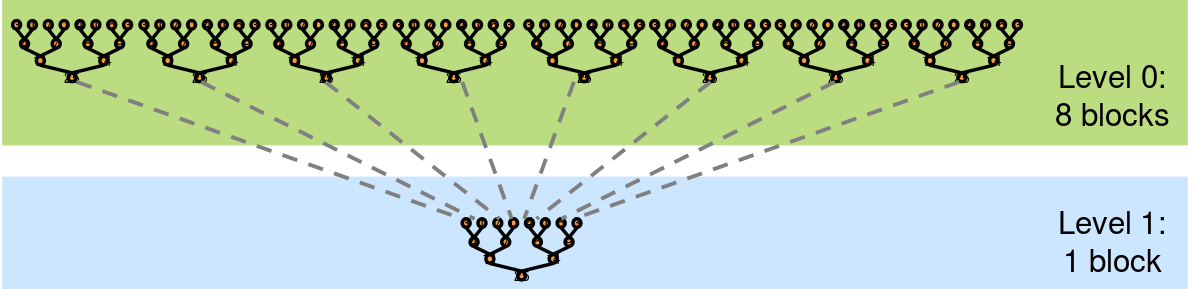
\includegraphics[width=.8\textwidth]{images/reduce_decomp_example.png}
  \caption{Reducing over multiple sweeps}
  \label{fig:reduce decomp example}
\end{figure}

The idea is that each block in the image is performed by each kernel invocation.
\Cref{lst:reduce par} shows the reduce kernel.
The needed indices are calculated, followed by the block's reduction in the loop.
Before proceeding the code makes sure that all threads have finished.
Finally, only the first thread writes the block's reduction to the output array.
The output is written to the block's index in the grid, which makes sure that each block's result is written to independent addresses.

\begin{lstlisting}[caption={Reduce kernel}, label={lst:reduce par}]
__global__
void reduce_kernel(int *d_out, int *d_in, int SIZE) {
  int mid = threadIdx.x + blockIdx.x * blockDim.x,
      tid = threadIdx.x;

  for (int s = blockDim.x / 2; s > 0; s /= 2) {
    if ((tid < s) && ((mid + s) < SIZE))
      d_in[mid] += d_in[mid + s];
    __syncthreads();
  }

  if ((tid == 0) && (mid < SIZE))
    d_out[blockIdx.x] = d_in[mid];
}
\end{lstlisting}

The intermediate results are thus transferred to the next iteration of kernel invocations.
We add a wrapper function, in \cref{lst:reduce wrapper}, that runs these kernels iteratively.
We introduce temporary arrays to hold the intermediate results, and update the grid size number of elements accordingly before invoking the kernel again.
Finally, the code performs a final invocation of the kernel with the desired final output array to combine the results.

\begin{lstlisting}[caption={The loop in the wrapper for the reduce kernel}, label={lst:reduce wrapper}]
do {
  reduce_kernel<<<grid_size, BLOCK_SIZE>>>(d_tmp_out, d_tmp_in, size);
  // Updating intermediate arrays
  size  = grid_size;
  bytes = sizeof(int) * size;
  cudaMemcpy(d_tmp_in, d_tmp_out, bytes, cudaMemcpyDeviceToDevice);
  // Updating to reflect how many blocks we now want to compute on
  grid_size = size / BLOCK_SIZE + ((size % BLOCK_SIZE)?1:0);
} while(size > BLOCK_SIZE);
// Computing remainder
reduce_kernel<<<1, size>>>(d_out, d_tmp_out, size);
\end{lstlisting}

\subsection{Using Shared Memory}
\label{sec: reduce shared memory}

A rather quick optimisation is to use shared memory instead of global memory in the kernel.
The kernel performs read and write operations in the l
If we have 1024 threads per block then we will do more than 3000 read and write operations to global memory.
However, if we read the needed memory into shared memory and perform the loop on that memory, then we will do about 1000 read and write operations.
Thus, we can achieve a theoretical 3x speed up.
The number of read and writes are presented in \cref{tab:reduce global to shared}.

\begin{table}[htb]
  \centering
  \begin{tabular}{c r | r r r r r}
    \toprule
    \multirow{2}*{global memory} & read  & 1024 & 512 & 256 & $\cdots$ & 1 \\
                                 & write &  512 & 256 & 128 & $\cdots$ & 1 \\
    \midrule
    \multirow{2}*{shared memory} & read  & 1024 & & &  &  \\
                                 & write &    1 & & &  &  \\
    \bottomrule
  \end{tabular}
  \caption{Global vs. Shared memory read and writes}
  \label{tab:reduce global to shared}
\end{table}

We present the revised reduce kernel with shared memory in \cref{lst:reduce par shared}.
We add the \ttt{sdata} array to contain the shared memory, and each thread copies the global data to that shared memory.


\begin{lstlisting}[caption={Reduce kernel using shared memory}, label={lst:reduce par shared}]
__global__
void reduce_kernel(int *d_out, int *d_in, int SIZE) {
  int mid = threadIdx.x + blockIdx.x * blockDim.x,
      tid = threadIdx.x;
  if (mid >= SIZE) return;

  extern __shared__ int sdata[]; // allocate shared memory
  sdata[tid] = d_in[mid];        // each thread loads global to shared memory
  __syncthreads();               // make sure all threads are done

  for (int s = blockDim.x / 2; s > 0; s /= 2) {
    if ((tid < s) && ((mid + s) < SIZE))
      sdata[tid] += sdata[tid + s]; // perform operations on shared memory
    __syncthreads();
  }

  if ((tid == 0) && (mid < SIZE))
    d_out[blockIdx.x] = sdata[0];   // copy shared back to global memory
}
\end{lstlisting}

\begin{lstlisting}[caption={Updated call to reduce kernel after use of shared memory}, label={lst:reduce invocation with smem}]
const unsigned int SMEM = BLOCK_SIZE * sizeof(int);
reduce_kernel<<<grid_size, BLOCK_SIZE, SMEM>>>(d_tmp_out, d_tmp_in, size);
\end{lstlisting}

Furthermore, we must update the kernel call to include the amount of shared memory to be allocated.
This is illustrated in \cref{lst:reduce invocation with smem}, where the third argument in the triple chevrons is the amount of shared memory to allocate

We present a plot in \cref{fig:reduce plot} illustrating the development of the run time for the reduce algorithms presented.
The GPGPU gets an advantage when the array size to sum is large.
This is most likely due to that fact that the CPU is much faster than the GPGPU.
The GPGPU beats the CPU when it has enough work to spread out to its threads.

\begin{figure}[htb]
  \centering
  \section{Reduce}
\label{sec:reduce}

Another handy algorithm is the reduce algorithm.
The idea is to perform some binary operation on the collection of elements in some array, and return a single result.
This operation could for instance be a sum over all elements, where the operation would be addition.
The operation must be associative, i.e. \ttt{(a op b) op c = a op (b op c)}, for the reduce algorithm to perform correctly.
\Cref{lst:reduce seq} shows the serial reduce code.
The operation loops through all input elements and sums the result.

\begin{lstlisting}[caption={Serial reduce}, label={lst:reduce seq}]
void reduce(int *h_in, int h_out, int SIZE) {
  for (int l = 0; l < SIZE; ++l) 
    h_out += h_in[l];
}
\end{lstlisting}

The challenge with the reduce code is that we perform all operations on a single memory address.
If the serial code is naively made parallel we have a race condition.
We need to split the problem into smaller problems and perform several sweeps on the results and combine the intermediary results to get the final result.
We present an illustration in \cref{fig:reduce decomp example} to try to give an intuition of how the parallel code will run.~\cite{reduceharris}

\begin{figure}[htb]
  \centering
  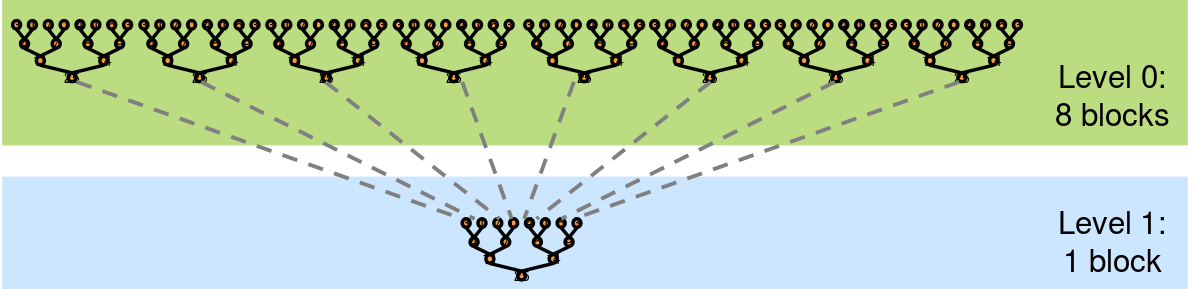
\includegraphics[width=.8\textwidth]{images/reduce_decomp_example.png}
  \caption{Reducing over multiple sweeps}
  \label{fig:reduce decomp example}
\end{figure}

The idea is that each block in the image is performed by each kernel invocation.
\Cref{lst:reduce par} shows the reduce kernel.
The needed indices are calculated, followed by the block's reduction in the loop.
Before proceeding the code makes sure that all threads have finished.
Finally, only the first thread writes the block's reduction to the output array.
The output is written to the block's index in the grid, which makes sure that each block's result is written to independent addresses.

\begin{lstlisting}[caption={Reduce kernel}, label={lst:reduce par}]
__global__
void reduce_kernel(int *d_out, int *d_in, int SIZE) {
  int mid = threadIdx.x + blockIdx.x * blockDim.x,
      tid = threadIdx.x;

  for (int s = blockDim.x / 2; s > 0; s /= 2) {
    if ((tid < s) && ((mid + s) < SIZE))
      d_in[mid] += d_in[mid + s];
    __syncthreads();
  }

  if ((tid == 0) && (mid < SIZE))
    d_out[blockIdx.x] = d_in[mid];
}
\end{lstlisting}

The intermediate results are thus transferred to the next iteration of kernel invocations.
We add a wrapper function, in \cref{lst:reduce wrapper}, that runs these kernels iteratively.
We introduce temporary arrays to hold the intermediate results, and update the grid size number of elements accordingly before invoking the kernel again.
Finally, the code performs a final invocation of the kernel with the desired final output array to combine the results.

\begin{lstlisting}[caption={The loop in the wrapper for the reduce kernel}, label={lst:reduce wrapper}]
do {
  reduce_kernel<<<grid_size, BLOCK_SIZE>>>(d_tmp_out, d_tmp_in, size);
  // Updating intermediate arrays
  size  = grid_size;
  bytes = sizeof(int) * size;
  cudaMemcpy(d_tmp_in, d_tmp_out, bytes, cudaMemcpyDeviceToDevice);
  // Updating to reflect how many blocks we now want to compute on
  grid_size = size / BLOCK_SIZE + ((size % BLOCK_SIZE)?1:0);
} while(size > BLOCK_SIZE);
// Computing remainder
reduce_kernel<<<1, size>>>(d_out, d_tmp_out, size);
\end{lstlisting}

\subsection{Using Shared Memory}
\label{sec: reduce shared memory}

A rather quick optimisation is to use shared memory instead of global memory in the kernel.
The kernel performs read and write operations in the l
If we have 1024 threads per block then we will do more than 3000 read and write operations to global memory.
However, if we read the needed memory into shared memory and perform the loop on that memory, then we will do about 1000 read and write operations.
Thus, we can achieve a theoretical 3x speed up.
The number of read and writes are presented in \cref{tab:reduce global to shared}.

\begin{table}[htb]
  \centering
  \begin{tabular}{c r | r r r r r}
    \toprule
    \multirow{2}*{global memory} & read  & 1024 & 512 & 256 & $\cdots$ & 1 \\
                                 & write &  512 & 256 & 128 & $\cdots$ & 1 \\
    \midrule
    \multirow{2}*{shared memory} & read  & 1024 & & &  &  \\
                                 & write &    1 & & &  &  \\
    \bottomrule
  \end{tabular}
  \caption{Global vs. Shared memory read and writes}
  \label{tab:reduce global to shared}
\end{table}

We present the revised reduce kernel with shared memory in \cref{lst:reduce par shared}.
We add the \ttt{sdata} array to contain the shared memory, and each thread copies the global data to that shared memory.


\begin{lstlisting}[caption={Reduce kernel using shared memory}, label={lst:reduce par shared}]
__global__
void reduce_kernel(int *d_out, int *d_in, int SIZE) {
  int mid = threadIdx.x + blockIdx.x * blockDim.x,
      tid = threadIdx.x;
  if (mid >= SIZE) return;

  extern __shared__ int sdata[]; // allocate shared memory
  sdata[tid] = d_in[mid];        // each thread loads global to shared memory
  __syncthreads();               // make sure all threads are done

  for (int s = blockDim.x / 2; s > 0; s /= 2) {
    if ((tid < s) && ((mid + s) < SIZE))
      sdata[tid] += sdata[tid + s]; // perform operations on shared memory
    __syncthreads();
  }

  if ((tid == 0) && (mid < SIZE))
    d_out[blockIdx.x] = sdata[0];   // copy shared back to global memory
}
\end{lstlisting}

\begin{lstlisting}[caption={Updated call to reduce kernel after use of shared memory}, label={lst:reduce invocation with smem}]
const unsigned int SMEM = BLOCK_SIZE * sizeof(int);
reduce_kernel<<<grid_size, BLOCK_SIZE, SMEM>>>(d_tmp_out, d_tmp_in, size);
\end{lstlisting}

Furthermore, we must update the kernel call to include the amount of shared memory to be allocated.
This is illustrated in \cref{lst:reduce invocation with smem}, where the third argument in the triple chevrons is the amount of shared memory to allocate

We present a plot in \cref{fig:reduce plot} illustrating the development of the run time for the reduce algorithms presented.
The GPGPU gets an advantage when the array size to sum is large.
This is most likely due to that fact that the CPU is much faster than the GPGPU.
The GPGPU beats the CPU when it has enough work to spread out to its threads.

\begin{figure}[htb]
  \centering
  \input{graphics/plots/reduce}
  \caption{Runtime development of three reduce algorithms}
  \label{fig:reduce plot}
\end{figure}

We mentioned that the shared memory version of the reduce would theoretically get approximately a 3x speed-up compared to the regular version.
This is not the case as illustrated in the plot.
This is due to the fact that we do not utilize the full potential of the local memory of the device.
If we were to get closer to the theoretical speed-up we would have to do more optimisations.

  \caption{Runtime development of three reduce algorithms}
  \label{fig:reduce plot}
\end{figure}

We mentioned that the shared memory version of the reduce would theoretically get approximately a 3x speed-up compared to the regular version.
This is not the case as illustrated in the plot.
This is due to the fact that we do not utilize the full potential of the local memory of the device.
If we were to get closer to the theoretical speed-up we would have to do more optimisations.

  \caption{Runtime development of three reduce algorithms}
  \label{fig:reduce plot}
\end{figure}

We mentioned that the shared memory version of the reduce would theoretically get approximately a 3x speed-up compared to the regular version.
This is not the case as illustrated in the plot.
This is due to the fact that we do not utilize the full potential of the local memory of the device.
If we were to get closer to the theoretical speed-up we would have to do more optimisations.

  \caption{Runtime development of three reduce algorithms}
  \label{fig:reduce plot}
\end{figure}

Using amdahls law would conclude that this problem is not as parallelizable as the mapping function from the previous section and should thus achieve a lesser speed-up.
At $n=2^{29}$ the CPU performs the reduce in $1332.38ms$ where as the GPGPU performs the global reduce in $165.92$, x$8.03$ speed-up, and shared reduce in $124.07$, x$10.74$ speed-up.

We mentioned that the shared memory version of the reduce would theoretically get approximately a 3x speed-up compared to the regular version.
This is not the case as illustrated in the plot and by the speed-ups.
This is due to the fact that we do not utilize the full potential of the local memory of the device.\cite{udacity}
